%%%%%%%%%%%%%%%%%%%%%%%%
%%%%%%%%% Préambule %%%%%%%%%
%%%%%%%%%%%%%%%%%%%%%%%%
\documentclass[a4paper,12pt]{article}
\usepackage{etex}

%%%%%Langue%%%%%

%%\usepackage[utf8]{inputenc}

\usepackage[T1]{fontenc}
\usepackage{babel} 
%%%%Police%%%%

 %% MATHS BELLES : \usepackage{mathpazo}
 %% TIMES NEW ROMAN :
\usepackage{stmaryrd}
\usepackage{newtxtext, newtxmath}
%%%%%Packages%%%%%

\usepackage[dvipsnames]{xcolor}

\usepackage{afterpage,amsfonts,amsmath,amssymb,amsthm,array,cancel,caption,comment,diagbox,dsfont,enumitem,fancybox,fancyhdr,float, framed,graphics,graphicx,hhline,import,latexsym,lscape,mathabx,multicol,multirow,pdfpages, setspace,subcaption,systeme,tikz,url,xcolor,mdframed}

\usepackage[left=2.5cm, right=2.5cm, top=2.5cm, bottom=2.5cm]{geometry}
\onehalfspacing
\usepackage[french,boxruled]{algorithm2e}
\usepackage[colorlinks=true]{hyperref} 
\usepackage[all]{xy}
\usepackage{dashundergaps}
\usepackage{pgfplots}
\usepackage{pdfpages}
\pgfplotsset{compat=1.18, width=10cm}
\dashundergapssetup{gap-extend-minimum=20pt,gap-extend-percent=20, gap-numbers=false,gap-format=dot,gap-widen=true,teacher-gap-format=dot}

\setlength{\columnsep}{0cm}

\usetikzlibrary{shapes.misc}
\newcommand{\mytimes}{ \tikz[baseline=-.55ex] \node [inner sep=0pt,cross out,draw,line width=1.5pt,minimum size=0.75ex] (a) {};}

\usepackage{tcolorbox}
\tcbuselibrary{theorems}

%%%%Couleurs%%%%

%Version en ligne

\definecolor{t2_red}{RGB}{210,12,70}
\definecolor{t2_blue}{RGB}{12,128,210}
\definecolor{t2_gold}{RGB}{210,180,12}
\definecolor{wooclap_blue}{RGB}{108,151,243}
\definecolor{t2}{RGB}{144,93,146}

%Version Imprimable

%\definecolor{t2_red}{RGB}{0,0,0}
%\definecolor{t2_blue}{RGB}{0,0,0}
%\definecolor{t2_gold}{RGB}{0,0,0}
%\definecolor{wooclap_blue}{RGB}{0,0,0}
%\definecolor{t2}{RGB}{0,0,0}

\hypersetup{urlcolor=t2_red,linkcolor=t2_red,citecolor=t2_red,colorlinks=true}


%%%%%Environnements%%%%%

\newtcbtheorem[number within=section]{defi}{Définition\,}{colback=t2_red!0,colframe=t2_blue,fonttitle=\bfseries}{df}

\newtcbtheorem[number within=section]{prop}{Proposition\,}{colback=t2_red!0,colframe=t2_red,fonttitle=\bfseries}{prop}

\newtcbtheorem[number within=section]{cor}{Corollaire\,}{colback=t2_red!0,colframe=t2_red,fonttitle=\bfseries}{cr}

\newtcbtheorem[number within=section]{theo}{Théorème\,}{colback=t2_red!0,colframe=t2_gold,fonttitle=\bfseries}{th}

\theoremstyle{definition}
%\newtheorem{conv}{Convention}
\newtheorem*{defin}{Définition}
\newtheorem*{ex}{Exemple}
\newtheorem*{exo}{Exercice}
\newtheorem*{corr}{Correction}
\newtheorem*{rap}{Rappel}
\newtheorem*{rem}{Remarque}
\newtheorem*{que}{Question}
\newtheorem*{rems}{Remarques}
\theoremstyle{plain}
\newtheorem*{conj}{Conjecture}
\newtheorem*{demo}{Démonstration}
%\newtheorem{cor}{Corollaire}
%\newtheorem{princ}{Principe}
\newtheorem*{lem}{Lemme}
%\newtheorem{prop}{Proposition}
%\newtheorem{theo}{Théorème}
%\newtheorem*{theo_non_numero}{Théorème}

%%%%%%Algorithmes%%%%%
\newcommand{\ulesalgorithm}[2]{%
	\vspace{1cm}
	\fbox{\parbox{\textwidth}{%
			{\bf #1}\\[2mm]
			{\tt #2 }
	}}
	\vspace{1cm}
}


\newcommand{\blobb}[1]{%
	\begin{list}{$\bullet$}{%
			\setlength{\topsep}{0cm}
			\setlength{\partopsep}{-\parskip}
			\setlength{\leftmargin}{0.5cm}
		}{\item #1}%
	\end{list}
}
%\declaretheorem[name=Proposition,sibling=prop]{proprep}

%%%%%Macros%%%%%

%%Ensembles%classiques%%

\def\N{\mathbb{N}}%entiers naturels
\def\Z{\mathbb{Z}}%entiers relatifs
\def\Q{\mathbb{Q}}%rationnels
\def\R{\mathbb{R}}%réels
\def\C{\mathbb{C}}%complexes

%%Algèbre%linéaire%%
\def\1char{\mathbb{1}}
\def\codim{\mathrm{codim}}%codimension
\def\ker{\mathrm{ker}\,}%noyau
\def\coker{\mathrm{coker}\,}%conoyau
\def\im{\mathrm{im}\,}%image
\def\id{\mathrm{id}}%application identité
\newcommand\scal[2]{\langle #1,#2\rangle}%produit scalaire

%%Géométrie%différentielle%%

\def\grad{\mathrm{grad}}%gradient
\def\ind{\mathrm{ind}\,}%indice
\def\modu{\mathcal{M}}%espace de modules
\def\moduc{\overline{\mathcal{M}}}%espace de modules compactifié
\def\moducbullet{\overline{\mathcal{M}_\bullet}}%espace de modules avec un point marqué compactifié
\def\ev{\mathrm{ev}}%applications évaluations dans la base
\def\Ev{\mathrm{Ev}}%applications évaluations dans l'espace total
\def\lacet{\ell}%lacet de Morse
\def\lacets{\mathcal{L}}%lacets de Morse
\newcommand\ro{roulement}%roulement-crocodile
\newcommand\Star{{S_\star}}%ensemble du point étoilé et des augmentations
\newcommand\fibrEv{\underset{\Ev}{\boxtimes}}%produit fibré des évaluations dans l'espace total
\newcommand\fibrev{\underset{\mathrm{ev}}{\boxtimes}}%produit fibré des évaluations dans la base
\newcommand\moducmix[1]{\overline{\modu^{#1}}}%espace de modules mixtes
\newcommand\moducmixbul[1]{\overline{\modu^{#1}_\bullet}}%espace de modules à rebonds
\newcommand\moducprime{\overline{\mathcal{M}'}}%espace de modules pour un second jeu de données
\newcommand\rg{\mathfrak{r}}
\newcommand\qg{\mathfrak{q}}
\newcommand\Loop{\mathcal{L}}
\newcommand\push{\Phi}
\newcommand\drum{drumroll}

%%%%%Commandes%%%%%

\def\;{\,\,;\,\,}%point virgule espacé

\def\tq{\,\,\mathrm{t.q.}\,\,}%tel que

\def\iff{\Longleftrightarrow}%équivaut à, la commande initiale ne marche pas

\def\implies{\Longrightarrow}%implique, la commande initiale ne marche pas

\newcommand\fonction[5]{#1:
	\begin{array}{ccc}
		#2&\longrightarrow &#3\\
		#4&\longmapsto &#5
\end{array}}%fonction avec ensembles de départ, d'arrivée et transformation

\newcommand\fonctionbira[5]{#1:
	\begin{array}{ccc}
		#2&\dashrightarrow &#3\\
		#4&\longmapsto &#5
\end{array}}

\newcommand\fonctionnonnommee[4]{\begin{array}{ccc}
		#1 &\longrightarrow& #2\\
		#3 &\longmapsto & #4
\end{array}}%fonction avec ensembles de départ, d'arrivée et transformation, sans nom


%%%%Tables%%%%
\usepackage{adjustbox}
\usepackage{booktabs}



%%%%%Bibliographie%%%%%

\bibliographystyle{alpha-en}

%%%%%Style%%%%%

\pagestyle{empty}
\pagestyle{fancy}

\setlength{\headheight}{16pt}
\usepackage{listings}

\definecolor{darkWhite}{rgb}{0.94,0.94,0.94}

\lstset{
	aboveskip=3mm,
	belowskip=-2mm,
	backgroundcolor=\color{darkWhite},
	basicstyle=\footnotesize,
	breakatwhitespace=false,
	breaklines=true,
	captionpos=b,
	commentstyle=\color{red},
	deletekeywords={...},
	escapeinside={\%*}{*)},
	extendedchars=true,
	framexleftmargin=16pt,
	framextopmargin=3pt,
	framexbottommargin=6pt,
	frame=tb,
	keepspaces=true,
	keywordstyle=\color{blue},
	language=C,
	literate=
	{²}{{\textsuperscript{2}}}1
	{⁴}{{\textsuperscript{4}}}1
	{⁶}{{\textsuperscript{6}}}1
	{⁸}{{\textsuperscript{8}}}1
	{€}{{\euro{}}}1
	{é}{{\'e}}1
	{è}{{\`{e}}}1
	{ê}{{\^{e}}}1
	{ë}{{\¨{e}}}1
	{É}{{\'{E}}}1
	{Ê}{{\^{E}}}1
	{û}{{\^{u}}}1
	{ù}{{\`{u}}}1
	{â}{{\^{a}}}1
	{à}{{\`{a}}}1
	{á}{{\'{a}}}1
	{ã}{{\~{a}}}1
	{Á}{{\'{A}}}1
	{Â}{{\^{A}}}1
	{Ã}{{\~{A}}}1
	{ç}{{\c{c}}}1
	{Ç}{{\c{C}}}1
	{õ}{{\~{o}}}1
	{ó}{{\'{o}}}1
	{ô}{{\^{o}}}1
	{Õ}{{\~{O}}}1
	{Ó}{{\'{O}}}1
	{Ô}{{\^{O}}}1
	{î}{{\^{i}}}1
	{Î}{{\^{I}}}1
	{í}{{\'{i}}}1
	{Í}{{\~{Í}}}1,
	morekeywords={*,...},
	numbers=left,
	numbersep=10pt,
	numberstyle=\tiny\color{black},
	rulecolor=\color{black},
	showspaces=false,
	showstringspaces=false,
	showtabs=false,
	stepnumber=1,
	stringstyle=\color{gray},
	tabsize=4,
	title=\lstname,
}

\usepackage[pages=some]{background}

\backgroundsetup{
	scale=1,
	color=black,
	opacity=1,
	angle=0,
	contents={%
		\includegraphics[width=\paperwidth,height=\paperheight]{"figures/PDG_V0"}
	}% %Userpackage for background
}

%%%%%En-tête%%%%%
\date{June 7, 2024.}
\begin{document}

\BgThispage
\begin{titlepage}
	\centering
	\vspace*{3cm}
	{\large LAAS-CNRS.\\
		April 29th - June 14th, 2024.
		\par}
	\rule{0.6\textwidth}{2pt}\\
	{\huge\bfseries Internship report : \\ Evaluation of Spectral Clustering methods. \\\par}
	\rule{0.6\textwidth}{2pt}\\
	\vspace{2cm}
	{\large
		HACINI Malik
		\par }
	\vspace{1cm}
	{\Large\bfseries Supervised by\par} \:
	{\large JONCKHEERE Matthieu\par}
	
\end{titlepage}

\begin{abstract}
	During my internship at LAAS-CNRS in Toulouse, I focused on exploring and implementing Spectral Clustering algorithms. This report begins with an introduction to the laboratory and outlines the objectives of my internship. I then delve into the technical aspects, starting with an overview of the fundamental theory behind Spectral Clustering. Following this, I describe my implementation of the algorithm in Python and detail the experiments conducted on synthetic datasets to evaluate its performance.
	
	The report further introduces Generalized Spectral Clustering (GSC), a novel framework developed at LAAS. I explain the theoretical ideas and improvements offered by GSC over traditional Spectral Clustering methods. To test and demonstrate the efficacy of GSC, I present experiments performed on both synthetic and real-life datasets.
	
	Overall, this report provides a comprehensive analysis of Spectral Clustering techniques, from basic theory to practical implementation and experimentation, culminating in an exploration of the advanced Generalized Spectral Clustering framework.
	

\end{abstract}
\newpage
\section*{Thanks}
I would like to express my heartfelt gratitude to everyone who supported me during my internship at LAAS-CNRS. Firstly, I am deeply thankful to my supervisor, Matthieu Jonckheere, for his unwavering support and guidance. His willingness to allow me to work independently while providing insightful guidelines made this internship a truly enriching experience. I am particularly grateful for the opportunity he gave me to explore a field I am passionate about, which has been incredibly rewarding.

I also sincerely thank Ernesto Garcia, Ph.D. student, whose office I shared. Ernesto was always there to patiently answer my questions, offer valuable insights, and share his experiences about the world of academic research and its challenges. His support and willingness to help made a significant difference in my learning journey.

Additionally, I would like to thank Jérome Monnier, Pascal Noble, Aude Rondepierre, and Lucie Baudoin for connecting me with Matthieu and providing me with this valuable opportunity. Your belief in my potential and your efforts to facilitate this internship have been crucial.

I am also deeply grateful to my sponsor teacher, Jean Marc Hok, who gave me the opportunity to write this report in English. This experience allowed me to fully immerse myself in the academic world, enhancing my understanding and skills in scientific writing.

Lastly, I wish to extend my sincere thanks to "La Prépa des INP," my school, for giving me the opportunity to undertake this internship.

\newpage
\tableofcontents
\newpage
\section{Introduction}
Clustering data is crucial in various fields as it allows us to identify patterns, group similar entities together and derive meaningful insights from large datasets. In virtually every
scientific field dealing with empirical data, people attempt to get a first impression on their data by
trying to identify groups of “similar behavior” in their data. These fields include machine learning where it is referred to as unsupervised learning, healthcare where clustering techniques are used to identify groups of patients with similar medical characteristics facilitating the conducting of studies and marketing where clustering allows businesses to segment customers based on arbitrary chosen criteria, often used to personalize advertisement. To perform clustering, algorithms are built using mathematical tools from probability theory, statistics, linear algebra and functional analysis.\\ A classic approach is the $k$-means algorithm, which aims at partitioning the data into $k$ predefined clusters centered at specific points and minimizing within-cluster variances. However, this problem is computationally NP-Hard and although efficient heuristics exist, $k$-means performs poorly on datasets with inadequate geometry or very high dimensional ones. Moreover, the number $k$ of clusters need to be known before performing the algorithm, which can be a big problem.
A new theoretical framework for clustering has developed in the past 25 years with the goal of overcoming these limitations. It aims to identify clusters based on the similarity between data points. It views the data points as nodes in a graph and analyzes the graph's structure to partition the data. This analysis uses spectral properties of the graph, leading to the name of \textbf{spectral clustering}.
In the last 3 decades, spectral clustering has become one of the most widely used clustering methods  due to its simplicity, efficiency, and strong theoretical background.
\begin{figure}[H]
	\centering
	\includegraphics[width=0.7\linewidth]{figures/Fig1}
	\caption{Comparison between $k$-means clustering and spectral clustering on a toy dataset}
	\label{fig:fig1}
\end{figure}
However, due to it's relative recency and important practical applications, spectral clustering is still heavily studied today. It still has theoretical limitations that hinders it's performance. Improving the theory behind these algorithms is the goal of a team of researchers at LAAS-CNRS in Toulouse. This report presents the internship I have done in their team over the course of 6 weeks.\\
The goal of the internship was understanding classical spectral clustering (SC) in theory, then dive into \textbf{generalized spectral clustering} (GSC), the renewed theory of SC that the team is working on. I could then try helping the team by implementing SC and GSC on synthetic and real datasets, aiming to conduct experiments on the performance of these algorithms. This would hopefully lead to guiding theoretical research towards methods with the best experimental results, as good experimental results may be the sign of the existence of good theoretical results. \\
This internship allowed me to reinvest the mathematical tools learned during La Prépa in an Applied Mathematics context. To deeply understand the theory of SC and GSC, I also had to learn new mathematics, mostly in probability theory and functional analysis. I was also able to practice my Python programming skills and learn the art of presenting experimental results in a scientific way.
Most importantly, I was fully involved in the team, working at the lab and sharing everyday with it's researchers from all around the globe, discovering the world of academics.

\section{An overview of LAAS-CNRS}
LAAS-CNRS is a french research lab of the \textit{Centre National de la Recherche Scientifique} (CNRS), the biggest public research organism in France.
LAAS stands for \textit{Laboratoire d'analyse et d'architecture des systèmes} (Laboratory of system analysis and architecture). Behind this rather complex acronym lies 4 historical disciplinary fields : computer science, robotics, automatics and micro and nano systems.
The 'systems' considered in LAAS' research activites are of diffrent kinds :integrated systems, robotic systems, biological systems... \\
They fall in various application domains such as aeronautics and space, telecommunications, transports, production, services, security and defense, energy management, healthcare, environment and sustainable development.

\subsection{Foundation}
LAAS was created in 1968 under the name \textit{Laboratoire d'automatique et de ses applications spatiales} (Laboratory of automatics and it's spatial applications). Indeed, it is located in Toulouse, a leading city in spatial technology, near other important academic entities such as ENAC or CNES (National Centre for Space Studies).
\begin{figure}[H]
	\centering
	\includegraphics[width=0.4\linewidth]{figures/LAAS}
	\caption{LAAS-CNRS Facility in Toulouse}
	\label{fig:laas}
\end{figure}
\subsection{Lab organization and philosophy}
LAAS is the home of 6 research departments made up of 26 teams dedicated to their 4 disciplinary fields.
All departments combined, over 800 people work at LAAS, including 200 permanent researchers and 230 PhD students.
\begin{figure}[H]
	\centering
	\includegraphics[width=0.6\linewidth]{figures/LAAS_Departments}
	\caption{LAAS' 6 research departments.}
	\label{fig:laasdepartments}
\end{figure}
The lab has a history of strong relationships with industry and works in a large number of collaborative projects with international, national and regional industries of all size. LAAS was one of the 20 first “Carnot Institutes” labeled in 2006, a label given to labs putting an emphasis on industry partnership.
LAAS also takes great advantage of it's pluridisciplinary nature : teams from different departments often collaborate to build projects. LAAS promotes transdisciplinary research through 4 strategic axes: Ambient intelligence, Living (biology, environment, medicine), Space and Energy. Examples include LAAS' mathematicians teaming up with robotics researchers to provide efficient Machine Learning (ML) algorithms for their projects.

\subsection{SARA}
During my internship, I was integrated in the SARA research team, short for "Services and Architectures for Advanced Networks". The SARA team works on new-generation networks and communication systems. The team is mostly made up of experts in networks and communication, and mathematicians focused on ML and applied probability. I was mostly working with Director of Research Matthieu Jonckheere and P.h.D students Ernesto Garcia and Vittorio Puricelli, as they are involved in the subject of the internship.

\section{Internship's details }
I worked daily in the office of Ernesto Garcia, where I could easily communicate with the him and Vittorio. The goal was to evaluate different Spectral Clustering methods, specifically the GSC framework developed by the team, by conducting experiments of the behavior of these methods for synthetic and real datasets. For this, I had to implement an unsupervised SC / GSC pipeline in Python. This theoretical framework was built on ideas that the team thought could potentially improve clustering in certain scenarios, and we wanted to test these ideas in practice.
This work can be broken down in $3$ big steps : 
\begin{itemize}
	\item Theoretical Understanding of SC and GSC
	\item Implementation of the algorithms in Python
	\item Conduct of experiments on synthetic and real datasets
\end{itemize}
In practice, these $3$ steps intertwined a lot : I understood the algorithms more and more as I was implementing them, while conducting experiments every step of the way.

\section{The theory of Spectral Clustering}
The first task I was given was to understand the theory of classical spectral clustering by reading \cite[A tutorial on Spectral Clustering]{tutorial}, the most famous introductory article on the subject. SC has been heavily studied for the past $3$ decades, and this article does a great job at introducing the theory and giving practical advice on the algorithm. Later on, I would have to establish specific experiments myself, thus a superficial understanding would not be enough and I had to deeply understand the mechanisms of the algorithm. The theory of SC is mostly built using graph theory and linear algebra. It is then interpreted by the theory of Markov processes on graphs. I was already familiar most of the mathematical material required, up to some advanced linear algebra results like the Perron-Frobenius theorem. I also had to deepen my understanding of the Markov chain approach to random walks to get a better feel for the inner mechanisms of GSC.
It took me $4$ days to understand the basics and start working on my first implementation of SC, but I refined my understanding day by day afterwards.
\subsection{Technical explanation} \label{sec-theory}
Since I will later present the results of my experiments, a technical explanation on the basics of spectral clustering will be useful. For more details, see \cite{tutorial}.
Let $S$ be a set of $N$ data points $x_1,x_2, \ldots ,x_N$ in $\R^n$.
\subsubsection{Similarity graphs}
The main idea of spectral clustering is to represent the data points as the nodes (or vertices) of a "similarity graph". The first step is choosing a distance/similarity symmetric function $d: \R^n \mapsto \R$ that defines pairwise distances $w_{ij} = d(x_i,x_j)$ between every point of the set .

\begin{itemize}
	\item $k$-nearest neighbors graph
	\item $\varepsilon$-neighborhood graph
	\item Fully connected graph
\end{itemize}
The $k$-nearest neighbors graph connects (via edges) every point to it's $k$ nearest neighbors in the dataset relative to $f$. It is an unweighted directed graph. \\
The $\varepsilon$ graph connects two points $(p_1,p_2)$ if and only if $w_{ij} < \varepsilon$ where $\varepsilon > 0$  is a treshold. It is an unweighted undirected graph. \\
The fully connected graph simply connects every point with every other one, weighing all edges by $w_{ij}$. Thus, it is a weighted undirected graph. \\

The end goal is to detect clusters in the set, so the graph should represent the local neighborhood relationships between points. Thus, the fully connected construction is only useful if $d$ models the local neighborhoods. An example for such a similarity function is the Gaussian similarity function $d(x_i,x_j)=exp(\frac{-\lVert x_i - x_j \rVert)^2}{é\sigma^2})$, where the parameter σ controls the width of the neighborhoods. This parameter plays a similar role as the parameter $\varepsilon$ in the case of the $\varepsilon$-neighborhood graph.
For $k$-nn and $\varepsilon$-neighboorhood graphs, the classical euclidean distance can also be used.\\

There are very few theoretical results on the question of how the choice of the similarity function/graph influences the spectral clustering result. However, the SARA team studies clustering with $k$-nn graphs and they are easier to work with in practice, thus I will only consider this type of graph in the rest of this work.
Here is an example of the $k$-nn gaph of a $2$ dimensional dataset :

\begin{figure}[H]
	\centering
	\includegraphics[width=0.6\linewidth]{figures/simgraph_example}
	\caption{$4$-nearest neighboirs similarity graph of a toy dataset;}
	\label{fig:sg_example}
\end{figure}
\begin{rem}
	In this specific example, the graph is undirected. This is not the case in general : a point $x_i$ can be in the $k$-nearest neighbors of another point $x_j$, but $x_j$ might not be one of the $k$-nearest neighbors of $x_i$. This is actually a problem, and it is adressed in the next section.
\end{rem}
\subsubsection{Graph laplacians}
The main tool used for spectral clustering is the "graph laplacian". It is a matrix traditionally defined using the adjacency matrix $W=(w_{ij})_{i,j=1,\ldots,N}$ \footnote{In the case of an unweighted graph, $w_{ij}=1$ if the edge $(x_i,x_j)$ exists and $0$ if it doesn't.} of the set's graph, called the similarity matrix, and the degree matrix $D=(d_i)_{i \in {1,\ldots N}}$ where $d_i=\sum_{j=1}^{N}w_{ij}$ is the degree of the vertex $x_i$.

There exists no unique "graph laplacian". Instead, multiple matrices are referred to as "graph laplacians" in the litterature.The most common ones are :
\begin{itemize}
	\item The unnormalized laplacian $L = D - W$
	\item The first normalized laplacian $L_{sym}=D^{-1/2}LD^{-1/2}$
	\item The second normalized laplacian, also called random walk laplacian $L_{rw}= I - D^{-1}W$
\end{itemize}

If we were asked to cluster the data from the previous example, we would create $2$ obvious clusters : the points on the left and the points on the right. A point in one of these clusters is very close to other points of the cluster, compared to points on the other side. Thus, it is only connected to points of the same cluster : the $2$ clusters are disconnected.
The similarity graph has $2$ connected components, each of them being a cluster. 
In general, we can define a cluster as an isolated subset of points that are close to each other, but relatively far to the rest of the set. Thus, in the ideal case of completely separated clusters, detecting clusters is the same thing as detecting the connected components of the similarity graph. \\
This is the main idea of spectral clustering, and graph laplacians are built for this task.
\begin{theo*}{Number of connected components and spectra of the graph laplacians} \label{con_theo}
	Let $G$ be an undirected graph with
	non-negative weights. Then the multiplicity $k$ of the eigenvalue
	$0$ of $L$, $L_{rw}$ and $L_{sym}$ equals the number of connected
	components $A_1, \hdots, A_k$ in the graph. The eigenspace of $0$ is
	spanned \footnote{for $L_{sym}$ it is actually spanned by $D^{1/2} \1char_{A_i}$, but the consequences are the same.} by the indicator vectors $\1char_{A_i}$ of those
	components.
\end{theo*}

\begin{proof}
	See \cite{tutorial}.
\end{proof}
This theorem implies that computing the eigenspace of $0$ of the graph laplacian gives us all the information about the connected components of the similarity graph : their number (by the multiplicity), and the nodes in them (by the eigenvectors). We can then build an algorithm to cluster the data based on this information. We give this algorithm with the unnormalized laplacian $L$.

\ulesalgorithm{Unnormalized spectral clustering}{
	Input: Similarity matrix $W \in \R^{n \times n}$, number $k$ of clusters to con\-struct. 
	\blobb{ Construct a similarity graph. Let $W$ be its weighted adjacency matrix. }
	\blobb{Compute the unnormalized Laplacian $\Lun$. }
	\blobb{{\bf Compute the first  $\boldsymbol k$ eigenvectors $\boldsymbol{u_1,\hdots,u_{k}}$ of $\boldsymbol{L}$.} }
	\blobb{ Let $U \in \R^{n \times k}$ be the matrix containing the vectors $u_1,\hdots,u_k$ as
		columns. }
	\blobb{ For $i=1,\hdots,n$, let $y_i \in \R^{k}$ be the vector corresponding to the $i$-th
		row of $U$. }
	\blobb{ Cluster the points $(y_i)_{i=1,\hdots,n}$ in $\R^k$ with the $k$-means
		algorithm into clusters $C_1,\hdots,C_k$. }
	Output: Clusters $A_1,\hdots,A_k$ with  $A_i = \{j | \; y_j \in C_i\}$.}
	
Applied to the previous example, we get exactly what we wanted :
\begin{figure}[H]
	\centering
	\includegraphics[width=0.6\linewidth]{figures/clustering_example}
	\caption{Spectral clustering of a toy dataset with an undirected similarity graph with $2$ disconnected components.}
	\label{fig:c_example}
\end{figure}

The previous theorem is very powerful, but relies on $2$ major hypothesis that flaws the perfection of this theoretical spectral clustering.
\paragraph{The importance of directionality} 
The connectivity theorem holds only for undirected graphs. Why ? \\
An undirected graph is defined by $w_{ij}=w_{ji}$, thus $W$ is a real symmetric matrix. This leads to the graph laplacians being real symmetric positive semi-definite matrices which ensure they have non-negative real eigenvalues. This is crucial for establishing the theorem. \\ However, we have stated $k$-nn to be the most intersting construction of a similarity graph, but it can lead to directed graphs, which would break the theory apart. The classical naive way to deal with this problem is to artificially symmetrize $W$ using $\frac{1}{2}(W + W^{T})$. This simply ignores the directions of the edges, that is we connect $v_i$ and $v_j$ with an undirected edge if $v_i$
is among the k-nearest neighbors of $v_j$ or if $v_j$ is among the k-nearest neighbors of $v_i$. \\
However, this may discard valuable information regarding the directionality of the graph. This is the problem that led the SARA team to work on a renewed SC theory, detailed in \cite{GSC}.

\paragraph{The case of disconnected clusters} 
The first example given is the "ideal case". For most real datasets, clusters will not be as well separated, and there will be links between clusters. 
\begin{figure}[H]
	\centering
	\includegraphics[width=0.6\linewidth]{figures/connected_example}
	\caption{Connected similarity graph of a toy dataset. The color of the points represent the ground truth. }
	\label{fig:connected_example}
\end{figure}
In this case, the graph possesses exactly $1$ connected component, as it is fully connected. Thus, the eigenspace of $0$ is of dimension $1$ and is spanned by $(1,\ldots,1) \in \R^n$, and it seems we cannot use this information to cluster the data.
However, in practice, SC is done exactly like described, even for these datasets. How does it work ? \\
There are multiple lines of reasoning trying to explain the efficacy of SC. We will only present one, see \cite{tutorial} for more details and other approaches.
\paragraph{Perturbation theory approach} 
Perturbation theory studies the question of how eigenvalues and
eigenvectors of a matrix $A$ change if we add a small perturbation
$H$, that is we consider the perturbed matrix $\tilde A := A + H$.
Most perturbation theorems state that a certain distance between
eigenvalues or eigenvectors of $A$ and $\tilde A$ is bounded by a
constant times a norm of $H$. The constant usually depends on which
eigenvalue we are looking at, and how far this eigenvalue is separated
from the rest of
the spectrum (for a formal statement see below). 
%
The justification of spectral clustering is then the following: Let us
first consider the ``ideal case'' where the between-cluster similarity
is exactly 0. Then, as stated by \ref{con_theo}, the first $k$ eigenvectors of $L$ or $L_{rw}$ are the indicator
vectors of the clusters. In this case, the points $y_i \in \R^k$
constructed in the spectral clustering algorithms have the form
$(0,\hdots,0,1,0,\hdots0)'$ where the position of the 1 indicates the
connected component this point belongs to. In particular, all $y_i$
belonging to the same connected component coincide. The $k$-means
algorithm will trivially find the correct partition by placing a
center point on each of the points $(0,\hdots,0,1,0,\hdots0)' \in
\R^k$.
%
In a ``nearly ideal case'' where we still have distinct clusters, but
the between-cluster similarity is not exactly 0, we consider the
Laplacian matrices to be perturbed versions of the ones of the ideal
case. Perturbation theory then tells us that the eigenvectors will be
very close to the ideal indicator vectors. The points $y_i$ might not
completely coincide with $(0,\hdots,0,1,0,\hdots0)'$, but do so up to
some small error term. Hence, if the perturbations are not too large,
then $k$-means algorithm will still separate the groups from each
other. \\
\paragraph{The eigengap heuristic}
In the ideal case of disconnected clusters, we know the multiplicity of the eigenvalue $0$ to be the number of connected components, thus of clusters in this framework. However, in more complex scenarios, $0$ will only have a multiplicity of $1$. But in theory at least, we can still use the spectra of the graph laplacian to detect the correct number of clusters. Indeed, according to perturbation theory, for a set with $k$ clusters, it's $k$ first eigenvalues (in ascending order) should be very close to $0$, and the next one further away from it. Thus, we should be able to see a "gap" in the spectra after the $k$ first eigenvalues. The quantity $\lvert \lambda_{k+1} - \lambda_k \rvert$ is thuscalled the eigengap. \\
In practice, this heuristic is hard to use : we do not have much control over the spectra of the graph laplacians apart from the eigenvalue $0$, and do not know much about the parameters that influence this eigengap.\\ Identifying these parameters and trying to improve the eigengap was one of the main focus of the experiments \ref{sec-exp} conducted during this internship.
\section{Python implementation of SC}
There already exists multiple Python implementations of SC, the most notable being the one used in the \cite[scikit learn]{scikit} package. However, this implementation has limited customization and does not include the GSC framework. Thus, I had to implement SC from scratch on my own. This was done using only standard Python libaries such as NumPy and SciPy. The code was split in $2$ main modules : one being responsible for the creation and management of similarity graphs and their laplacians, and the other being in charge of the actual clustering. On top of that, I added a tool for building datasets. It consists of an interactive matplotlib window where one can place points in $2$D space in real time, and assign them colors that will serve as the ground truth label of the dataset. This tool was crucial, as it made running experiments on synthetic data way easier and faster.
\begin{figure}[H]
	\centering
	\includegraphics[width=0.6\linewidth]{figures/dataset_builder}
	\caption{The dataset builder.}
	\label{fig:dataset_builder}
\end{figure}
I also included the GSC framework in the library, detailed in \ref{sec-gsc}. This implementation had $2$ major goals : being highly customizable (every parameter of the clustering can be freely chosen), to easily conduct experiments, but also being usable in an unsupervised way. \\
The only information needed to run SC on a dataset is the number of clusters. Every other parameter, if not given, is chosen automatically. For details, see \ref{app-unsupervised}. \\
I have then compiled the library into an installable open-source Python package named GSCpy. Using it requires no particular knowledge on SC, and the dataset builder is included. For details, see the \cite[GSCpy github repository]{github}.
\section{Spectral Clustering Experiments} \label{sec-exp}

Before diving into the theory of GSC and the experiments, I conducted several experiments on classical SC to assert the good behavior of the algorithms and weigh the impact of certain parameters.
\subsection{Basic Experiments}
\subsubsection{Circles and Moons}
The most basic spectral clustering example are the circles and moons dataset. These datasets fail to be clustered correctly by $k$-means, as the clusters do not lie in disjoint convex sets. However, spectral clustering is powerful enough to correctly cluster these datasets, as the clusters form disconnected components in the graph. This shows the philosophical advantage that SC has : it doesn't care about the dataset's geometry.

\begin{figure}[H]
	\begin{subfigure}{.6\textwidth}
		\centering
		\includegraphics[width=0.9\linewidth]{figures/Fig1}
		\caption{Circles}
	\end{subfigure}
	\begin{subfigure}{.6\textwidth}
		\centering
		\includegraphics[width=0.9\linewidth]{figures/Fig2}
		\caption{Moons}
	\end{subfigure}
	\caption{Comparison between $k$-means and spectral clustering on toy datasets}
\end{figure}


Here, we know the correct number of clusters because we can visualize the dataset, which is not the case for real datasets as they are highly dimensional. However, as predicted by the theory, the spectra of the graph laplacian is helpful.


\begin{figure}[H]
	\captionsetup{justification=centering}
	\centering
	\includegraphics[width=1.1\linewidth]{figures/Fig_E1_circles}
	\caption{First eigenvalues of laplacians for the clustering of the circles dataset. \\ Left to right : $L$, $L_{sym}$, $L_{rw}$}
	\label{fig:fige1circles}
\end{figure}

Every laplacian has a great gap in it's eigenvalues after 2 of them, meaning the graph contains exactly 2 connected components, thus 2 clusters.
In order to show the difference between each laplacian, we need more sophisticated datasets.

\subsubsection{Gaussian Mixtures}
Before implementing the dataset builder, which came late in the process of the internship, I had to build datasets on my own using other ways. Matthieu and Ernesto suggested that in the goal of doing qualitative comparison between different methods, using $2$-dimensional gauussian mixture datasets would be a good starting point. 

\paragraph{Multivariate Normal Distribution} The multivariate normal distribution, also called "multivariate gaussian" is a generalization of the one-dimensional (univariate) normal distribution to higher dimensions. For any dimension $d$, it can be defined by it's PDF :
$$\fonctionnonnommee{\R^{d}}{\R_{>0}}{x}{\frac{1}{\sqrt{(2\pi)^2 \lvert \Sigma \rvert}} e^{-\frac{1}{2}(x-\mu) \Sigma^{-1} (x-\mu)^{t}}}$$
Where:
\begin{itemize}
	\item $\mu \in{R^d}$ is the mean of the distribution.
	\item $\Sigma$ is a $d$ by $d$ square symmetric positive semi-definite matrix called the covariance matrix, because when $x$ is treated as a random vector with each of it's coordinates $x_i$ being a random variable, $\sigma_{i,j}= Cov(x_{i},x_{j})$.
\end{itemize}
The multivariate gaussian distribution is centered at $\mu$ and has an ellipsoidal shape defined by $\Sigma$.
\begin{figure}[H]
	\centering
	\includegraphics[width=0.4\linewidth]{figures/Binorm}
	\caption{Level sets of a bivariate normal distribution centered at the origin. The probability of a sample landing in the blue ellipse is $0.66$.}
	\label{fig:binorm}
\end{figure}

A linear combination of $d$-dimensional gaussians is called a gaussian mixture.
\begin{figure}[H]
	\centering
	\includegraphics[width=0.6\linewidth]{figures/2gm}
	\caption{$200$ samples from a mixture of two 2-dimensional gaussians.}
	\label{fig:2gm}
\end{figure}
\begin{rem} 
	In practice, since gaussians PDF decay quickly when driving away from $\mu$, when the means are fairly spaced, the different gaussians do not really interact to form a diffrent PDF and the resulting mixture just looks like a superpostion of the respective gaussians. Thus, we do not perform the sampling with the actual PDF of the mixture, but uniformly choose between the different gaussians for each point.
\end{rem}
Gaussian mixtures form great toy datasets on which we can test and visualize our clustering, where a "ground truth" cluster is all of the points sampled from a particular gaussian.

\begin{figure}[H]
	\captionsetup{justification=centering}
	\begin{subfigure}{.6\textwidth}
		\centering
		\includegraphics[width=0.9\linewidth]{figures/fig5_g1}
		\caption{Successful clustering}
	\end{subfigure}
	\begin{subfigure}{.6\textwidth}
		\centering
		\includegraphics[width=0.9\linewidth]{figures/fig6_g2}
		\caption{Unsuccessful clustering}
	\end{subfigure}
	\caption{Visualization of spectral clustering and it's $k$-nn graph on a gaussian mixture. \\ Settings : $L_{rw}$, $k=6$, $\sigma=\frac{1}{3}$ (for gaussian kernel).}
\end{figure}
On figure (a) we see that the $k$-nn graph correctly encodes the cluster structure of the data. It is fully connected but there is only one link between clusters, which makes for great performance of SC using $L_{rw}$. \\ \\
On figure (b), the means of the two gaussians are closer apart, thus the clustering fails to partition the graph correctly due to the multiple links between the real clusters.
However, increasing $k$ creates stronger links inside of the clusters, leading to better performance : 
\begin{figure}[H] 
	\label{unsuc}
	\centering
	\includegraphics[width=0.6\linewidth]{figures/fig7_g3}
	\caption{The performance of the clustering is increased with $k=8$}
	\label{fig:fig7g3}
\end{figure}
By forcing the algorithm to form $2$ clusters, we get good performance. Again, what if we didn't know the true number of clusters ? In this case, the graph is fully connected, so does the eigengap really indicates $2$ clusters ? 

\begin{figure}[H]
	\captionsetup{justification=centering}
	\begin{subfigure}{.3\textwidth}
		\centering
		\includegraphics[width=1.1\linewidth]{figures/Fig_E4_L}
		\caption{$L$}
	\end{subfigure}
	\begin{subfigure}{.3\textwidth}
		\centering
		\includegraphics[width=1.1\linewidth]{figures/Fig_E5_L_sym}
		\caption{$L_{sym}$}
	\end{subfigure}
	\begin{subfigure}{.3\textwidth}
		\centering
		\includegraphics[width=1.1\linewidth]{figures/Fig_E6_L_rw}
		\caption{$L_{rw}$}
	\end{subfigure}
	\caption{First eigenvalues of laplacians for the graph of \ref{unsuc}.}
\end{figure}
These results clearly show that the connectivity of the graph has great impact of the quality of the eigengap. Both the spectra of $L$ and $L_{rw}$ give no valuable information and while $L_{sym}$ does have a "gap" after the second eigenvalue, it isn't clear enough to conclude on the true number of clusters.
In conclusion, while the eigengap can be a useful criteria in the case of well separated datasets, when the graph is strongly connected to better the performance on harder datasets, the eigengap becomes meaningless as noise becomes too big.
Thus, we conclude that to efficiently choose $k$, we need to connect the graph enough to ensure good performance, but not too much to the point where the eigengap is useless, otherwise we will be unable to know the correct number of clusters. The practical implementation of this reasoning is detailed in \ref{app-unsupervised}.

\section{Generalized Spectral Clustering} \label{sec-gsc}
We have already underlined the theoretical limitations of spectral clustering in \ref{sec-theory}. Most importantly, in the classical process, we always lose the directionality information of the graph. This is what \cite[Jonckheere et al.]{GSC} tried to fix in their new framework : Generalized Spectral Clustering. The goal is to build a spectral clustering framework that would work on directed and undirected graphs. However, for this to work, we need a symmetric and real-valued graph Laplacian with a full set of real eigenvalues.\\ The bulk of the work is centered around the random walk interpretation of spectral clustering (See \cite{tutorial} for more details).A random walk on a graph is a stochastic process which randomly jumps from node to node.
We will see below that spectral clustering can be interpreted as trying to find a partition of the graph
such that the random walk stays long within the same cluster and seldom jumps between clusters.
Intuitively this makes sense, as when the intra-cluster links are stronger than the inter-cluster links, the random walk does not have
many opportunities to jump between clusters.
This leads to an expression of the spectral clustering problem as the relaxation of a functional of the graph, called \textit{generalized Dirichlet energy}. 
They are then able to build two new "generalized" laplacians, $L_{G}$ and $L_{G_{rw}}$. \\
In the case of a directed graph, these laplacians coincide with the standard $L$ and $L_{rw}$, hence the adjective "generalized". \\

\section{GSC Experiments}
The GSC framework has potential to improve SC, especially in the case of unbalanced data.\\
Jonckheere et al. have conducted experiments on GSC and found promising results. I was thus asked to pursue these experiments to try and better understand the behavior of GSC.
\subsection{Extensive study of the eigengap for SC and GSC}
\subsubsection{Method}
$k$ is not the only parameter with an impact on the eigengap. In this section we investigate characteristics of synthetic $2$-d datasets to assess their impact on the eigengap. In theory, the GSC framework involves new parameters $(t,\gamma,\alpha)$ used to build the generalized laplacians $L_{G}$ and $L_{G_{rw}}$. For this study, we fix $(t,\gamma,\alpha)$=$(3,0.7,0.9)$ for every dataset. To simplify the study, we first consider the case of $2$ clusters. We investigate $3$ features of the datasets:
\begin{itemize}
	\item Geometry of clusters
	\item $N$-symmetry
	\item Total number of points.
\end{itemize}
The big picture idea is to detect if clusters that "look alike" lead to better eigengaps, and if GSC improves them.
"Geometry of clusters" refers to the shape of the clusters. $2$ clusters are $N$-symmetric if they have the same number of points. We also call them 'balanced'.
To test these criteria, we generate multiple datasets and cluster them using every standard laplacian ($L$,$L_{sym}$,$L_{rw}$) and the generalized laplacians $L_G$ and $L_{G_{rw}}$. We make sure to separate these clusters well, to isolate the effect of our criteria on the eigengap. We are then able to choose $k$ efficiently by hand as the datasets are on the easier side. In practice, the standard laplacians return nearly identical results regarding performance of clustering and eigengap, thus we choose to only report $L_{rw}$ results and compare them to the generalized laplacians.
\subsubsection{Results}
\paragraph{Geometry of clusters.}
To correctly isolate the effect of the geometry of clusters, we build $N$-symmetric and $D$-symmeytric datasets. We start by a dataset with $2$ circular clusters to serve as reference.
We get the best results with $L_{G_{rw}}$.
\begin{figure}[H]
	\centering
	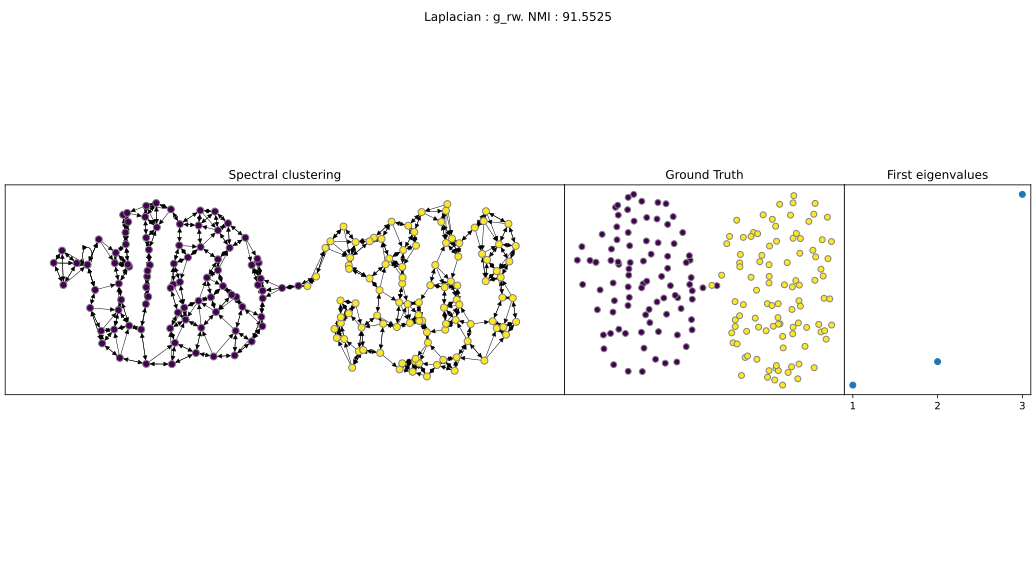
\includegraphics[width=0.6\linewidth]{figures/base_circles_g_rw}
	\label{fig:base_circles}
	\caption{$k$ = 4, $L_{G_{rw}}$. A great eigengap is observed.}
\end{figure}
As shown by the next experiment, changing the shape of one cluster doesn't change these results :
\begin{figure}[H]
	\centering
	\includegraphics[width=0.6\linewidth]{figures/uneven_blobs_g_rw}
	\label{fig:uneven_blobs}
	\caption{$k$ = 4, $L_{G_{rw}}$. An eigengap of the same quality is observed.}
\end{figure}

Other experiments allow us to conclude that the shape of the clusters has no significant impact on the performance of the clustering and the quality of the eigengap.
These results were to be expected : spectral clustering looks for the connected components of a $k$-nn graph. This graph does not contain the information of the shape of the clusters : in the adjacency matrix, a circular cluster will appear the same as an highly complex non-convex one. The underlying geometry of the subset of $\R^N$ a cluster belongs to is not taken into account when forming the graph. This is an advantage spectral clustering has over $k$-means, which looks for convex clusters in $\R^N$.\\
For the sake of simplicity and without loss of generality, we thus only consider circular clusters for our experiments on $N$-symmetry and the total number of points.
\paragraph{$N$-symmetry}
The \ref{fig:base_circles} dataset serves as a good example for $N$-symmetric clusters. The eigengap clearly indicates $2$ clusters.
This isn't true when the clusters are unabalanced.

\begin{figure}[H]
	\centering
	\includegraphics[width=0.6\linewidth]{figures/4x_asym_blobs_rw}
	\label{fig:mid_asym_blobs_rw}
	\caption{$k$ = 4, $L_{rw}$. There is $4$ times more points in the yellow cluster, the eigengap is worse.}
\end{figure}

\begin{figure}[H]
	\centering
	\includegraphics[width=0.6\linewidth]{figures/mid_asym_blobs_rw}
	\label{fig:4x_asym_blobs_rw}
	\caption{$k$ = 4, $L_{rw}$. There is $5$ times more points in the yellow cluster, the eigengap is practically unusable.}
\end{figure}
The more unbalanced the clusters are, the worse the eigengap. We conclude that for heavily unbalanced data, we can not safely rely on the spectra of the classical graph laplacians to detect the correct number of clusters.
GSC helps greatly for this matter.
\begin{figure}[H]
	\centering
	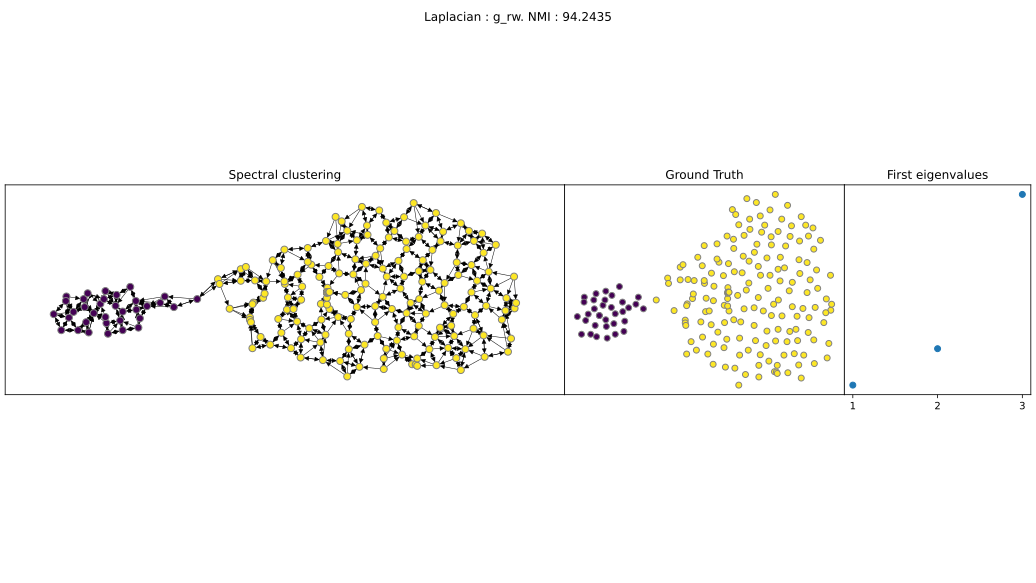
\includegraphics[width=0.7\linewidth]{figures/mid_asym_blobs_g_rw}
	\label{fig:mid_asym_blobs_g_rw}
	\caption{$k$ = 4, $L_{G_{rw}}$. Even with the data being heavily unbalanced, the eigengap is clear.}
\end{figure}
We can conclude that GSC leads to a better eigengap than classical SC on unbalanced data, which gives hope for the performance of a potentially fully unsupervised GSC pipeline, where the number of clusters is automatically detected by the algorithm.
\paragraph{Total number of points}
Most real datasets have a very high number of points, ranging from thousands to millions. Thus, in the hope of building a fully unsupervised GSC pipeline,asserting good eigengaps on large datasets is crucial.
Fortunately, experiments on synthetic datasets show that in general, more points lead to a better eigengap.
\begin{figure}[H]
	\centering
	\includegraphics[width=0.7\linewidth]{figures/circ_100_sym}
	\label{fig:circ_100_sym}
	\caption{$N=100$,$k$ = 4, $L_{G_{rw}}$. Points generated from a mixture of $2$ gaussians.}
\end{figure}
\begin{figure}[H]
	\centering
	\includegraphics[width=0.7\linewidth]{figures/circ_500_sym}
	\label{fig:circ_500_sym}
	\caption{$N=500$, $k$ = 4, $L_{G_{rw}}$. The eigengap is significantly better than with $100$ points. }
\end{figure}
These results hold for more and more points, although the rate of the upgrade in quality slows down over time.
\subsection{Real datasets}
SC and GSC is ultimately intended to be used for real datasets. Thus, I was asked to benchmark the algorithms on $10$ datasets from the \cite[UCI ML repository]{UCI} .

\subsubsection{Normalized Mutual Information (NMI)}
These datasets are high dimensional and to correctly assert performance of the clustering, we need a pertinent quantitative metric.
The NMI facilitates comparisons between two different ways of partitioning a dataset, yielding a value that ranges from 0 to 1. A higher value indicates a greater degree of similarity between partitions. As an external metric, the NMI necessitates the availability of class labels for computations, implying that the ground truth is required when employing this metric.
The calculation of the NMI between two partitions A and B is executed according to the following equation :
$$NMI\left(A,B\right)=\frac{2*I(A,B)}{[H\left(A\right)+H(B)]}$$

Where $I(A,B)$ is the mutual information and $H$ the entropy. 
In practice, $A$ is the set of predicted labels and $B$ the ground truth labels of the dataset. \\ NMI can fail to correctly assess the performance of the clustering when the number of clusters predicted and the ground truth number of clusters do not match. However, this won't be the case in our experiments, since we will force the clustering to build the right number of clusters.
Other evaluation metrics such as the adjusted Rand Index (ARI) exist, but we limited ourselves to NMI for these experiments as it already is very well suited for comparison purposes.
\subsection{Method and results}
We compare the $5$ graph laplacians : $L$, $L_{sym}$,$L_{rw}$,$L_{G}$ and $L_{G_{rw}} $. We construct a $k$-nn graph using the optimal connectivity parameter $k$ computed by \cite[Jonckheere et.al]{GSC} for each set. In the following results table, $N$ is the number of samples and $d$ their dimension.

\newcolumntype{L}[1]{>{\raggedright\let\newline\\\arraybackslash\hspace{0pt}}m{#1}}
\newcolumntype{C}[1]{>{\centering\let\newline\\\arraybackslash\hspace{0pt}}m{#1}}
\newcolumntype{R}[1]{>{\raggedleft\let\newline\\\arraybackslash\hspace{0pt}}m{#1}}
\renewcommand{\arraystretch}{1}
\setlength{\tabcolsep}{3pt}
%--
\begin{table*}[h]
	\small\centering
	\vspace{-3mm}
	\caption{Clustering performance (NMI) on UCI datasets with optimal parameters in brackets.}
	\label{tab_NMI_one}
	\vspace{-3mm}
	\sc
	\vskip 0.15in
	\begin{adjustbox}{width=0.6\textwidth,center}
		\begin{tabular}{L{25mm}R{8mm}R{5mm}R{5mm}||ccc||cc}
			\toprule
			Dataset & $N$ & $d$ & $k$ & $L$ & $L_{sym}$ & $L_{rw}$  & $L_{G}$ & $L_{G_{rw}}$ \\
			\midrule
			\midrule
			{Iris} & 150 & 3 & 4 &  80.58& 80.58& 74.98\\
			{Glass} & 214 & 9 & 6 & 38.59& 38.92&  38.95 \\
			{Wine} & 178 & 13 & 3 & 86.33& 86.33& 83.66\\
			{WBDC} & 569 & 30 & 2 & 67.73& 69.47& 68.54 \\
			{Control chart} & 600 & 60 & 6 & 81.17& 81.17& 82.94 \\
			{Parkinson} & 185 & 22 & 2 & 21.96& 19.13& 28.89 \\
			{Vertebral} & 310 & 6 & 3 & 39.26& 39.26&  52.06  \\
			{Breast Tissue} & 106 & 9 & 6 & 54.03& 54.43& 54.04  \\
			{Seeds} & 210 & 7 & 3 & 73.90& 73.90& 76.29 \\
			{Image Seg.} & 2310 & 19 & 7 & 67.06& 67.41 & 67.42\\
			{Yeast} & 1484 & 8 & 10 & 30.58& 31.11& 31.37	\\
			\midrule
			Average & -- & -- & -- & 58.29& 58.34& 59.92 \\
			\bottomrule
			%
		\end{tabular}
	\end{adjustbox}
	\vskip -0.1in
\end{table*}

TODO
\newpage
\appendix
\section{Unsupervised SC and GSC} \label{app-unsupervised}
TODO
\newpage

\begin{thebibliography}{9}
\bibitem{tutorial}Von Luxburg, U. A tutorial on spectral clustering. Statistics and
computing, 17(4):395–416, 2007.

\bibitem{UCI}
Dheeru, D. and Karra Taniskidou.UCI repository of machine learning databases \textit{University of California, Irvine, School of
	Information and Computer Sciences}, 2017.

\bibitem{GSC}
Harry Sevi, Matthieu Jonckheere, and Argyris Kalogeratos.
Generalized spectral clustering for directed and undirected graphs,
2022.

\bibitem{github}
\href{https://github.com/Malik-Hacini/GSCpy}{GSCpy : Generalized Spectral Clustering in Python.}
\bibitem{scikit} 
Scikit-learn: Machine Learning in Python, Pedregosa et al., JMLR 12, pp. 2825-2830, 2011.
\end{thebibliography}

\end{document}


